\documentclass[11pt,a4paper]{article}
\usepackage{hyperref}
\usepackage{emnlp2018}
\usepackage{times}
\usepackage{latexsym}
\usepackage{graphicx}
\usepackage{array}
\usepackage{float}
\usepackage{amsmath}

\usepackage{url}

\aclfinalcopy % Uncomment this line for the final submission

%\setlength\titlebox{5cm}
% You can expand the titlebox if you need extra space
% to show all the authors. Please do not make the titlebox
% smaller than 5cm (the original size); we will check this
% in the camera-ready version and ask you to change it back.

\newcommand\BibTeX{B{\sc ib}\TeX}
\newcommand\confname{EMNLP 2018}
\newcommand\conforg{SIGDAT}


\title{Project Laboratory}

\author{Csáky Richárd Krisztián \\}

\date{}

\begin{document}
\maketitle

\section{Introduction}
Current conversational models lack diversity and generate boring
responses to open-ended utterances \cite{Li:2015c,Wei:2017, Shao:2017b}.
{\it Priors} provide additional information to dialog models to
aid response generation, but annotating a dataset with priors such
as persona \cite{Li:2016a}, emotion
\cite{Zhou:2017}, or topic \cite{Xing:2017}, is expensive and such
annotations are rarely available. In this work a method is presented for improving
chatbots' responses to open-ended utterances by removing those
utterances from
training data using a simple entropy-based approach that
does not require human supervision. It is shown that training
on this filtered dataset results in better conversational quality as
chatbots learn to output better and more diverse responses to these
utterances.

A brief background and previous approaches to the issues mentioned are given in
Section~\ref{sec:background}, and Section~\ref{sec:methods} describes the
method in detail.
Section~\ref{sec:experiments} presents an analysis of the filtered
dataset, dialog systems trained on the new datasets are evaluated in
Section~\ref{sec:results}. Section~\ref{sec:conclusion} concludes and presents
future work. All code for the experiments in this paper can be found at \url{https://github.com/ricsinaruto/Seq2seqChatbots}.


\section{Background}
\label{sec:background}
\subsection{Chatbots}
A conversational agent (chatbot) is a piece of software that is able to communicate with humans using natural language. Many types of chatbots exist, but in this work the focus is on single-turn neural network based generative agents. Single-turn means that the only information the chatbot has is the previous utterance emitted by the user, and it has to form a reply based on this. Neural networks are widely used for modeling language \cite{Mikolov:2010}, and they have been shown to be capable of modeling dialog \cite{Vinyals:2015}. Finally, generative means that the chatbot is trying to emit replies that are not retrieved from some given dataset, but rather generated by the neural network model. Refer to \cite{Csaky:2017} for a more in-depth background on conversational agents.
\subsection{Neural Networks}
Neural networks are high-dimensional non-linear functions that can be used to model a plethora of tasks. Besides natural language they have been applied to image- and audio-based tasks as well \cite{Krizhevsky:2012, Van:2016}. In the chatbot case the neural network takes as input an utterance from a dialog dataset. The string utterance is transformed to a numerical representation using word vectors \cite{Mikolov:2013f}. The neural network takes these vectors as input and applies some mathematical transformations to produce an output. In the chatbot case the output is the response utterance to the given input. The exact type of mathematical transformations used is given by the architecture of the neural network. For conversational modeling some type of encoder-decoder model is used \cite{Sutskever:2014}. Neural network models have a plethora of parameters that can be changed inside the mathematical transformations. Through changing these parameters the right way a neural network can learn to produce better and better outputs, this being called learning or training. Essentially the output of the network is compared to the target output and based on the error, gradient descent is used to find the parameters inside the network that can best approximate the target output through an iterative process. Refer to \cite{Csaky:2017} for a more in-depth description of neural networks and their application to conversational modeling.
\subsection{Issues}
Current open-domain NCMs are based on neural architectures developed
for machine translation (MT). Conversational data differs
greatly from MT data in that targets to the same source sentence may vary not
only grammatically but also semantically
\cite{Wei:2017,Tandon:2017}; consider plausible replies to
the question: \textit{What did you do today?}. Dialogue datasets also
contain responses that appear after many different inputs, e.g. answers
such as \textit{yes}, \textit{no} and \textit{i don't
  know} appear after a large and diverse set of inputs.
Following the approach of modeling conversation as a sequence to sequence (\texttt{seq2seq})
\cite{Sutskever:2014} transduction of single dialog turns, these
issues can be referred to as the
\textit{one-to-many}, and \textit{many-to-one} problem, respectively. Since
\texttt{seq2seq} architectures are inherently deterministic, meaning that once trained
they can't output different sequences to the same input sequence, they are not
suited to deal with the ambiguous nature of dialogs.

The focus of this work is the \textit{one-to-many}, and \textit{many-to-one} problem,
previous approaches to which can be grouped into three
categories. First, the encoding procedure can be modified by feeding more
information into the model, like dialog history \cite{Serban:2015}, persona
information \cite{Li:2016a,Joshi:2017,Zhang:2018}, mood/emotion category
\cite{Zhou:2017,Li:2017b}, topic category \cite{Xing:2017, Liu:2017}, etc. Second, some approaches augment the decoding process, with
e.g. latent variable sampling \cite{Serban:2017b,Zhao:2017} or
beam search \cite{Goyal:2017,Wiseman:2016,Shao:2017b}. Finally, directly
modifying the loss function \cite{Wiseman:2016} or training procedure of the
model, by using reinforcement \cite{Li:2016b,
  Serban:2017a,Li:2016c,Lipton:2017} or adversarial learning \cite{Li:2017a} are also
  among the solutions proposed.

\section{Methods}
\label{sec:methods}
% clustering and filtering

In this work the \textit{one-to-many}, \textit{many-to-one} issue is
approached from a different perspective: instead of adding more complexity, we
try simple data filtering methods to exclude source-target utterance pairs
that have high entropy, since we believe that these cause dialog models to
output safe but boring responses. Entropy of utterances has also been used before for evaluation purposes \cite{Serban:2017b}. The entropy of a source/target utterance is
calculated based on the distribution of the target/source utterances that it
is paired with in the dataset. In essence, the learning task is formulated in
a way for which the maximizing likelihood approach is more suitable.
NCMs have been shown to produce better qualitative results after they overfit
the training data
\cite{Csaky:2017,Tandon:2017}. This also supports the claim that the loss
function is not capturing conversational goals, since a neural network model
should perform best when the validation loss is minimal. Our experiments
suggest that when training NCMs on our filtered datasets, validation loss
becomes a better indicator of the model's performance.

Of the 72 000 unique source utterances in the
DailyDialog dataset (see Section~\ref{sec:experiments} for details),
60 000 occur with only a single target. For these it seems
straightforward to maximize the conditional probability $P(T|S)$, $S$ and $T$ denoting
a specific source and target utterance.
However, in the case of sources that appear with multiple targets in the dataset,
models are forced to learn some ``average'' of
observed responses. This is the \textit{one-to-many} problem.
We can similarly formulate the \textit{many-to-one}
problem, where a diverse set of source utterances are observed with the
same target. This may be a less prominent issue in training NCMs,
since the probability of source utterances given some target
doesn't appear in standard loss functions (although it is used
in some special objective functions \cite{Li:2015c}). Still, we shall
experiment with excluding such targets (e.g. \textit{I don't know}),
since conversational models generate these quite frequently and they are
typically uninformative and unengaging (see Section~\ref{sec:eval} on
evaluation principles).

For each source utterance $s$ in the dataset we calculate the entropy
of the distribution $T|S=s$, i.e. given a dataset $D$ of source-target
pairs we define the
\textit{target entropy} of an utterance $s$ as 
\[ H_{\text{tgt}}(s, D) = - \sum_{(s, t_i)\in D} p(t_i|s)\log_2 p(t_i|s)
\]
Similarly, \textit{source entropy} of an utterance can be defined as
\[ H_{\text{src}}(t, D) = - \sum_{(s_i, t)\in D} p(s_i|t)\log_2 p(s_i|t)
\]
The probabilities are calculated based on the observed relative frequency of utterance pairs in the data. After calculating source and target entropies for each utterance in a
corpus, we filter the training data using one of 3 strategies. \textsc{target-based}, where pairs are filtered if the source utterance
has high target entropy. \textsc{source-based}, where
we filter based on the source entropy of the target utterance.
Finally, the \textsc{st-based} dataset is obtained by filtering pairs based on
both entropy values.


\section{Experiments}
\label{sec:experiments}
% actual filterings and trainings -> their results

\subsection{Dataset}
We use the DailyDialog
dataset\footnote{\url{http://yanran.li/dailydialog.html}} \cite{Li:2017b} in
our experiments. With 90 000 utterances in 13 000 dialogs, it is comparable in size
  with the Cornell Movie-Dialogs Corpus
\cite{Danescu:2011}, but contains real-world high quality dialogs, instead
of movie conversations, which are ``not truthful representations of real-life
conversations'' \cite{Danescu:2011}. The vocabulary was set to 16384, covering most of the words in the corpus (roughly 19000).

\subsection{Models}
For dialog modeling we use \texttt{transformer} \cite{Vaswani:2017}, a novel
encoder-decoder architecture. Compared to the standard recurrent neural
network (RNN) based \texttt{seq2seq} models, it doesn't use recurrent connections
and relies only on attention mechanisms \cite{Bahdanau:2015}. Consequently, it can
be trained much faster, and using less memory (training the
\texttt{seq2seq}
model of \cite{Vinyals:2015d} was not possible with the 8GB of GPU
memory we had access to). We further justify the use of this model with the fact that it achieves
state-of-the-art performance in NMT. Since the original \texttt{seq2seq} model was
adopted from NMT \cite{Cho:2014} to dialog modeling,
it is natural to do the same with the \texttt{transformer} architecture.
To justify its use for the dialog task, we also train a
\texttt{seq2seq} model (of limited size) on the same dataset for comparison.
The \texttt{transformer} and \texttt{seq2seq} models contain 53M and 317M
parameters, respectively. They are both large compared to the dataset thus
they easily overfit it, as will be shown in Section~\ref{sec:results}.
In the case of the \texttt{transformer} model we also experimented with different
dropout \cite{Srivastava:2014a} values our findings will also be
presented in Section~\ref{sec:results}.

We trained randomly initialized word embeddings (of size 512) together with the model parameters. Layer, attention, and relu dropout was set to 0.2, 0.1 and 0.1, respectively for the \texttt{transformer} model. At test time we used beam search with a beam size of 10 \cite{Graves:2012b}.

\subsection{Filtered data}
The 90 000 utterance pairs in the DailyDialog dataset contain about 72
000 unique utterances. We plot target entropies of source utterances in
Figure~\ref{fig:entropies}, ranked from lowest to highest entropy, not showing the majority of utterances which have 0 entropy (i.e. they do not appear with more than one target). Source entropies of target utterances are very similar. In the following
experiments we shall discard utterance pairs whose target and/or source entropy is greater
than 1. This affects 5.64\%, 6.98\% and 12.24\% of the data, for the \textsc{target-based}, \textsc{source-based} and \textsc{st-based} scenario, respectively.

\begin{figure}[!ht]
	\centering
	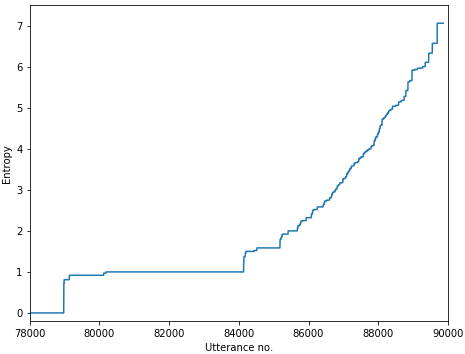
\includegraphics[width=0.47\textwidth]{pics/source_entropies.png}
	\caption{Source utterances by target entropy}
	\label{fig:entropies}
\end{figure}

Entropy is clearly proportional to utterance frequency
(Figure~\ref{fig:frequencies}), however we found that only 485 utterances overlap in the top 700 utterances (roughly what gets discarded) when ordered by both entropy and frequency, and those that are different in the frequency ordered list are long utterances, that we don't wish to filter out. Entropy offers a more fine-grained measure compared to frequency, and in the case of low frequency pairs, this is especially helpful. For example, all utterances that have a frequency of 3, are in the same category based on frequency, but their entropy can range from 0 to $\log_2 3\approx1.58$, which would be over our filtering threshold.



\begin{figure}[!ht]
	\centering
	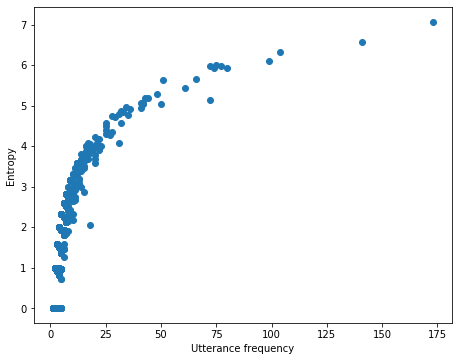
\includegraphics[width=0.47\textwidth]{pics/source_entropies_frequency.png}
	\caption{Target entropies of sources with respect to utterance frequency.}
	\label{fig:frequencies}
\end{figure}

After noticing that high-entropy utterances are relatively short, we
also examined the relationship between entropy and utterance length
(Figure~\ref{fig:length}). Given the relationship between frequency and
entropy it comes as no surprise that longer sentences have lower entropy,
although this effect is less pronounced in the range affected by filtering.

% and if they are unique then their
%entropy is 0, because the distribution consists of only 1 element.
\begin{figure}[!ht]
	\centering
	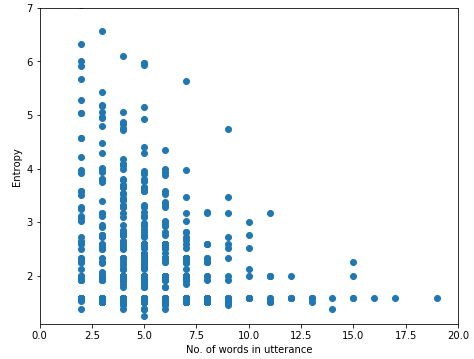
\includegraphics[width=0.47\textwidth]{pics/source_entropies_length.png}
	\caption{Target entropies of sources with respect to utterance length.}
	\label{fig:length}
\end{figure}

% ITT TARTOK (RG)
\section{Results}
\label{sec:results}
% compare \texttt{seq2seq} with transformer
% compare non-filtered and filtered trainings
% compare the different filtered trainings
% compare how overfitting affects the non-filtered and different filterings, for both models.
% also maybe show the top beams for the best filtered training and compare it with base
% Firstly a response has to be coherent, as much as a human response is. Only after it makes sense can we talk about whether it's boring or engaging
\subsection{Evaluation Principles}
\label{sec:eval}

Due to the limited scope of automatic evaluation
\cite{Liu:2016}, our claims are supported by both qualitative and quantitative evaluation of our models' outputs. We first summarize the principles used for
comparison, then present our findings.

We shall evaluate models based on answers they give to a list of input utterances.
When comparing responses given to the same question, we first consider
their \textit{coherence}, i.e. whether they could have been written by a
human speaker. Models that return coherent answers to an input
are further compared based on whether the answer is boring/generic (e.g.
\textit{I don't know}) or engaging/specific. 
Generic responses make sense in more dialog histories, however because of this
they do not add new information to the
conversation. More engaging responses, i.e. those that can further a conversation,
are preferred, but only if they are coherent with the source utterance.
While these principles, and thus our judgments presented here, are quite subjective,
we believe that the differences observed between various trainings
are sufficiently pronounced, and our findings are also grounded by the quantitative analysis.

Four metrics are used to quantitatively evaluate our models in Section~\ref{ssec:qa}. In order to measure the information content of a models' responses, average utterance length \(|U|\), word entropy \(H_w\) and utterance entropy \(H_u\) is computed \cite{Serban:2017b}. The entropies are computed with respect to the maximum-likelihood unigram distribution of the training set. Thus: \(H_w=-\sum_{w\in{U}} p(w)\log(p(w))\), and \(H_u\) is simply the product of utterance length and word entropy. Additionally the (string-based) average jaccard similarity \(J\) between source utterances and model responses is computed, measuring their coherence and relevance.  

\newcolumntype{p}[1]{>{\raggedright\let\newline\\\arraybackslash\hspace{0pt}}m{#1}}
\subsection{\texttt{seq2seq}, \texttt{transformer}, and overfitting}
\label{ssec:model_overfitting}
\begin{table*}[!ht]
	\fontsize{8}{12}\selectfont
	\renewcommand{\arraystretch}{0.6}
	
	\centering
	\begin{tabular}{
			>{\setlength{\baselineskip}{0.01\baselineskip}}p{2.5cm}
			>{\setlength{\baselineskip}{0.01\baselineskip}}p{3.5cm}
			>{\setlength{\baselineskip}{0.01\baselineskip}}p{3.5cm}
			>{\setlength{\baselineskip}{0.01\baselineskip}}p{1.5cm}
			>{\setlength{\baselineskip}{0.01\baselineskip}}p{2.5cm}}
		\textbf{Input} & \textbf{S2S-BASE} & \textbf{S2S-BASE-O} & \textbf{TRF-BASE} & \textbf{TRF-BASE-O} \\ \hline
		
		what 's your name ?&my name is james . my name is tiang .&\textbf{my name is wang lin . my english name is...CONT.}&\textbf{john .}&\textbf{my name is james .}\\ \hline
		when were you born ?&i was born in beijing . i was born .&i was born in beijing but i spent most of...CONT.&i was born in beijing .&i was born in .\\ \hline
		what year were you born ?&i was born in beijing . i was born .&i was born in beijing but i spent most of...CONT.&i was born in beijing .&i was born in xinjiang .\\ \hline
		where are you from ?&\textbf{i 'm from germany . how about you ?}&\textbf{i 'm from china . what about you ?}&i am from china .&i 'm from germany .\\ \hline
		are you a man or a woman ?&\textbf{i 'm not sure . what about you ?}&yes he is . he s climbing the tree .&i am .&he is five years old .\\ \hline
		why are we here ?&i do n't know what to say .&i do n't know . the weatherman did n't .&it looks good .&\textbf{it 's just near the dong si shi tiao subway...CONT.}\\ \hline
		my name is david . what is my name ?&this is mary .&my name is \textless unk\textgreater .&nice to meet you .&\textbf{hi david . nice to meet you .}\\ \hline
		my name is john . what is my name ?&this is mary .&my name is \textless unk\textgreater .&nice to meet you .&\textbf{hi lee . nice to meet you .}\\ \hline
		who is bill clinton ?&i do n't know . he 's a liar .&it 's martin scorsese . you liked his film .&that 's john .&that s the superintendent of this building .\\ \hline
		is sky blue or black ?&it 's a little tight in the back .&i 'm not sure . what about you ?&\textbf{black please .}&\textbf{white .}\\ \hline
		does a cat have a tail ?&yes of course . it s a good idea .&no he does n't . he 's an engineer .&yes we do .&as a matter of fact we have n't .\\ \hline
		does a cat have a wing ?&yes he does . he likes it very much .&yes he does . he is a science fiction writer...CONT.&\textbf{no they do n't .}&yes but not necessarily .\\ \hline
		can a cat fly ?&of course . that s a good idea .&yes they are . and driving is very good .&yes that 's right .&yes cats are fine . and they do n't need...CONT.\\ \hline
		how many legs does a cat have ?&i think it 's a good idea .&three . two boys and a pair of them .&about minutes .&oh come on . we have only one day .\\ \hline
		how many legs does a spider have ?&\textbf{let me see . . . here it is .}&\textbf{15 . and for a hard one only 6 .}&oh no .&only one year .\\ \hline
		what is the color of the sky ?&it 's the size of the size .&red . it 's made of fine leather shoes .&\textbf{it 's brown .}&it s a brandnew seiko wrist watch .\\ \hline
		what is the color of water ?&it 's the best we can do it .&leopard . it s famous for its quality only .&\textbf{it 's red .}&\textbf{it 's red .}\\ \hline
		what is the color of blood ?&it s the most important thing to me .&it is made of wood not plastic .&\textbf{it 's white .}&your doctor has requested a urine sample .\\ \hline
		what is the usual color of a leaf ?&it 's a \textless unk\textgreater .&it 's a \textless unk\textgreater with a vinyl roof .&\textbf{it 's white .}&\textbf{it 's blue .}\\ \hline
		what is the color of a yellow car ?&it 's a \textless unk\textgreater .&it 's a luminous watch with a \textless unk\textgreater function .&\textbf{it 's blue .}&\textbf{it 's a blue nissan minivan .}\\ \hline
		how much is two plus two ?&\textbf{let me see . . . here it is .}&15 . and for a hard one only 6 .&.&altogether .\\ \hline
		what is the purpose of life ?&i think it 's the most important thing to me...CONT.&i 'll be studying . i 'm doing an mba...CONT.&i 'm not sure yet .&for sightseeing .\\ \hline
		what is the purpose of living ?&i think it 's the most important thing to me...CONT.&i 'll be studying . i 'm doing an mba...CONT.&i 'm a personnel manager .&it 's a small family .\\ \hline
		where are you now ?&\textbf{on the second side of the campus .}&\textbf{i am on route 80 a few miles east .}&i 'm from canada .&\textbf{i am on route a few miles east of the...CONT.}\\ \hline
		what is the purpose of dying ?&\textbf{it s the most important thing to me .}&they have a really good dj and a big dance...CONT.&he is a lawyer .&\textbf{it takes a long time .}\\ \hline
		what is the purpose of being intelligent ?&the most important thing is the most important thing .&\textbf{i have no idea . i 'm impressed .}&i do n't know .&i do n't know .\\ \hline
		what is moral ?&\textbf{nothing .}&\textbf{pardon ?}&she 's a lawyer .&it is largest pop square in the world .\\ \hline
		give me some examples of moral actions . . .&what ?&so what ?&what 's wrong ?&anything else ?\\ \hline
		what is integrity ?&the most important thing is the most important thing .&you are suspected of hiding illegal drugs .&\textbf{the main thing is to people .}&the y . h . a . mun . the...CONT.\\ \hline
		be moral !&what ?&what 's the matter ?&what 's wrong ?&and your name ?\\ \hline
		what do you like to talk about ?&i do n't know what to say .&\textbf{i want to talk about this year s election .}&\textbf{i 'd like to talk to you about it .}&i do n't like her . ok .\\ \hline
		what do you think about bill gates ?&i think it 's a good idea .&\textbf{well i heard people say he has a bad cold...CONT.}&i 'm not sure .&\textbf{well he had a lot of nerve telling us this...CONT.}\\ \hline
		what is your job ?&i would like to work on my own .&i m a keyboard operator . what s your job...CONT.&i have worked as a personnel manager .&i 'm a bank manager .\\ \hline
		what do you do ?&i do n't know how to use it .&\textbf{i have my own company that designs computer systems .}&\textbf{i 'm a student .}&\textbf{i m a podiatrist . what about you ?}\\ \hline
		
	\end{tabular}
	\caption{Comparison between the two models (\texttt{seq2seq} and \texttt{transformer}) trained on unfiltered data,
		and between overfitted and non-overfitted variants. The input
		utterance is in the left-most column, the other columns contain
		responses by the various models. S2S and TRF represent \texttt{seq2seq} and
		\texttt{transformer} respectively, and the \textit{O} notation in the model
		name means that it is an overfitted version. In each row we highlighted the best responses.}
	\label{table:trf_s2s_compare}
\end{table*}

\begin{table*}[t!]
	\begin{center}
		\begin{tabular}{llll}
			
			\bf Unfiltered trainings & NCM test set & High entropy test set & NCM test set (2) \\ \hline
			
			\textsc{s2s-base} & 7 & - & - \\
			\textsc{s2s-base-o} & 9 & - & - \\
			\textsc{trf-base} & \textbf{\textit{11}} & 12 & 15 \\
			\textsc{trf-base-o} & \textbf{12} & - & - \\ \hline
			
			\bf Filtered trainings & & & \\ \hline
			\textsc{trf-st-based} & - & \textbf{23} & 15 \\
			\textsc{trf-st-based-o} & - & 7 & 13 \\
			\textsc{trf-target-based} & - & - & 11 \\
			\textsc{trf-source-based} & - & 11 & \textbf{16} \\ \hline
			
		\end{tabular}
	\end{center}
	\caption{\label{table:qualitative_numbers} Qualitative best response counts based on the different test sets. The test sets are the same as in the qualitative results. Since we evaluated separately the filtered and unfiltered trainings qualitatively there are two NCM test set columns. First, trainings which were trained on the normal (unfiltered) dataset are presented, and then trainings run on the filtered datasets. \textsc{trf} refers to the \texttt{transformer} model, and \textsc{s2s} refers to the \texttt{seq2seq} model. The type of filtering is also noted (\textsc{st-based}, \textsc{source-based}, \textsc{target-based}), and the \textsc{o} notation means that it is an overfitted version of the model. Results of best non-overfitted models are in italic boldface, while best results overall are noted by simple boldface.}
\end{table*}

We first compare overfitted and non-overfitted versions of the \texttt{seq2seq} (S2S) and
\texttt{transformer} (TRF) models trained on unfiltered data. Overfitted model versions,
are those that were trained further after the lowest value of validation loss
was reached, until training loss converges. We used a list of 34 general input utterances chosen from the ones used in \citet{Vinyals:2015d}, which we will call the NCM test inputs. We filtered this list by cutting well-known inputs to which each model learns to respond well (eg. \textit{Hello!}, \textit{How are you?}), and also removed inputs where any word was missing from the vocabulary.

For each input we determined the responses which we judged best, based on the
principles outlined at the beginning of this section (Table~\ref{table:trf_s2s_compare}). Also, we present the best response counts in Table~\ref{table:qualitative_numbers}, from which the first column is of relevance to this section. Generally,
the \texttt{transformer} performed better than the \texttt{seq2seq} model, achieving 11 best responses (among the 4 models), compared to only 7 for \texttt{seq2seq}. It managed to output colours when asked about the color of objects, while the \texttt{seq2seq}'s replies were irrelevant.

Overfitted models performed at least as well (in human evaluation) as non-overfitted models,
strengthening the points raised in \citet{Csaky:2017, Tandon:2017}: the loss
function does not adequately represent the quality of a chatbot model. The overfitted \texttt{seq2seq} model achieved 9 best responses (2 more than the non-overfitted version), and in the case of the \texttt{transformer} the overfitted version achieved 12 best responses. We note that overfitted models tend to generate longer responses, which is generally good, but in some cases we obtain too specific
and probably memorized responses to unrelated inputs (eg. \textit{they have a
  really good dj and a good dance.}  to the input \textit{what is the purpose of
  dying}).

Since our models overfit quickly, we also experimented with dropout.
With a high dropout rate (0.5) we can essentially force the validation loss to stay at its minimum
for longer, before starting to overfit. However, the minimum does not
go lower compared to low dropout (0.2) trainings, and the replies were generally the
same even after training more with high dropout, further consolidating
the observation
that the validation loss minimum does not represent the best state of the model.



\subsection{High Entropy Inputs}
\begin{table*}[!ht]
	\fontsize{8}{12}\selectfont
	\renewcommand{\arraystretch}{0.01}
	
	\centering
	\begin{tabular}{
			>{\setlength{\baselineskip}{0.01\baselineskip}}p{2cm}
			>{\setlength{\baselineskip}{0.01\baselineskip}}p{2.4cm}
			>{\setlength{\baselineskip}{0.01\baselineskip}}p{2.5cm}
			>{\setlength{\baselineskip}{0.01\baselineskip}}p{4cm}
			>{\setlength{\baselineskip}{0.01\baselineskip}}p{2.8cm}}
		\textbf{Input} & \textbf{TRF-BASE} & \textbf{TRF-FILTERED (\textsc{st-based})} & \textbf{TRF-FILTERED-O (\textsc{st-based})} & \textbf{TRF-FILTERED (\textsc{source-based})} \\ \hline
		
		yes .&how long have you been here ?&do you have any other ideas ?&what would you like for a drink ?&what 's your name ?\\ \hline
		certainly .&thank you very much .&\textbf{i 'm glad to hear that .}&ok so you are already a gold card holder with...CONT.&how about the lyrics ?\\ \hline
		yes please .&\textbf{how do you like it ?}&\textbf{how about this one ?}&here is your laundry . i am sorry to tell...CONT.&here is your laundry sir .\\ \hline
		yes ?&can you tell me how to use the machine ?&would you like to go with me ?&i was just thinking about someone i went to school...CONT.&what 's your name ?\\ \hline
		yes i do .&how do you like it ?&do you like it ?&what would you like for a drink ?&what 's your name ?\\ \hline
		here you are .&thank you .&do you have a receipt with you ?&would you please open the suitcase ? what are these...CONT.&here is your receipt .\\ \hline
		here you go .&thank you .&how much do you want to pay ?&do you have a credit card with us ?&here is your receipt .\\ \hline
		yes it is .&\textbf{how much is it ?}&\textbf{can you tell me how to use it ?}&we 're very sorry for the delay . i 'll...CONT.&what 's your name ?\\ \hline
		here it is .&thank you .&\textbf{how much is it ?}&\textbf{how much altogether ?}&here is your receipt .\\ \hline
		that 's right .&thank you .&\textbf{do you have any other ideas ?}&it must be very convenient and pretty quick .&how about the lyrics ?\\ \hline
		ok .&thank you .&\textbf{do you want to go with me ?}&and when we get back from the doctor 's you...CONT.&how about the lyrics ?\\ \hline
		okay .&thank you .&\textbf{do you want to go with me ?}&\textbf{so what were you calling me about ?}&how about the lyrics ?\\ \hline
		sure .&thank you .&\textbf{do you have any other ideas ?}&ok . . . i 'm just going to lay...CONT.&how about the lyrics ?\\ \hline
		i see .&thank you .&\textbf{would you like to go with me ?}&\textbf{which one interests you sir ?}&how about the lyrics ?\\ \hline
		all right .&thank you .&\textbf{do you have any other ideas ?}&the hair stylist cuts the customer 's hair . almost...CONT.&how about some fish ?\\ \hline
		no problem .&\textbf{thank you very much .}&i 'm sorry to hear that .&what is the price of the suite ?&how about the lyrics ?\\ \hline
		of course .&thank you very much .&\textbf{do you have any other ideas ?}&how about the lyrics ?&how about the lyrics ?\\ \hline
		what do you mean ?&you are suspected of hiding illegal drugs .&\textbf{i mean you 're right .}&when you take something out of the stores you need...CONT.&we 're stranded here tom .\\ \hline
		is that right ?&\textbf{yes that 's right .}&\textbf{yes that 's right .}&it must be very convenient...CONT.&yes that 's it .\\ \hline
		may i help you ?&yes i 'm looking for a pair of shoes .&i 'm looking for a sweater .&yes i 'm looking for a sweater .&yes i 'm looking for a sweater .\\ \hline
		how may i help you ?&i 'm looking for a pair of shoes .&i 'm looking for a sweater .&i need to open a second account .&i need to withdraw some money .\\ \hline
		what can i do for you ?&i 'm looking for a pair of shoes .&i 'm looking for a sweater .&well i 'm looking for a job .&i need to withdraw some money .\\ \hline
		is there anything i can do for you ?&\textbf{yes i 'm looking for a pair of shoes .}&yes i am . thank you very much .&\textbf{yes . i was looking for some help .}&\textbf{yes i 'm looking for a sweater .}\\ \hline
		anything else ?&\textbf{no that 's all .}&\textbf{no nothing else .}&i have taken some courses in college such as translation...CONT.&i 'd like to have some sweetandsour sauce and pepper .\\ \hline
		how much is it ?&yuan .&\textbf{59 . 95 .}&\textbf{55 dollars .}&\textbf{180 yuan .}\\ \hline
		how about this one ?&it looks good .&that 's fine . i 'll take it .&the style is all right but i 'm not sure...CONT.&it looks nice . how much is it ?\\ \hline
		really ?&yes .&yes it is .&yes and not expensive either .&yes it is .\\ \hline
		are you sure ?&yes i am .&yes i am .&yeah ! why not ? they are trendy and look...CONT.&yes i am sure i can .\\ \hline
		what ?&you are suspected of hiding illegal drugs .&\textbf{i 'm a vegan .}&a vegan . i do n't eat or use any...CONT.&what 's the matter with you ?\\ \hline
		why is that ?&i do n't know .&i do n't know .&because you can see the stars perfectly .&it 's just a waste of money .\\ \hline
		what 's that ?&it 's filthy !&\textbf{it 's a brick !}&well you know i have some students studying for their...CONT.&\textbf{it 's a kind of job .}\\ \hline
		what happened ?&i did n't know .&\textbf{it was nothing .}&i told you to get this consignment out last week...CONT.&\textbf{i went to the library .}\\ \hline
		what is it ?&\textbf{it 's a polo .}&\textbf{it 's a new car .}&it only has 4 beds and 4 writing desks but...CONT.&\textbf{it 's a polo . it has the logo on the back .}\\ \hline
		what 's the matter ?&i do n't know .&\textbf{i have a bad headache .}&\textbf{i 'm a little worried about my host family ....CONT.}&\textbf{my motherinlaw just went into the hospital in...CONT.}\\ \hline
		what seems to be the problem ?&i do n't know what to do .&i have been working on a business trip .&my roommate always brings a lot of friends from \textless unk\textgreater...CONT.&i have a problem with my work .\\ \hline
		why ?&i do n't know .&i have no idea .&well our public schools here are not very good and...CONT.&\textbf{it 's just a waste of money .}\\ \hline
		how come ?&\textbf{it does n't matter .}&not too bad .&my boss gave me a big project . i had...CONT.&\textbf{it 's too old .}\\ \hline
		why not ?&\textbf{it does n't matter .}&i do n't know .&video tape breaks down after fifteen years . so if...CONT.&\textbf{it 's just a waste of money .}\\ \hline
		like what ?&can you tell me how to use the internet ?&i like it very much .&i love you too .&how about the mongolian hot pot ?\\ \hline
		thank you very much .&\textbf{you 're welcome .}&\textbf{have a great day !}&please hold the line . i ll see if there...CONT.&\textbf{it 's my pleasure .}\\ \hline
		thanks a lot .&you 're welcome .&you 're welcome .&you are welcome&do n't mention it .\\ \hline
		thanks .&\textbf{you 're welcome .}&\textbf{you 're welcome .}&look ! here it is !&\textbf{you 're welcome . have a nice day .}\\ \hline
		no .&how about this one ?&how much is it ?&what did you do last night ?&how about the lyrics ?\\ \hline
		hello ?&yes what can i do for you ?&hi tom . how are you ?&no response silence&hello . this is john .\\ \hline
		good morning .&\textbf{good morning . can i help you ?}&\textbf{good morning ! can you help me please ?}&\textbf{good morning jamie . what time is it now ?}&may i help you ?\\ \hline
		
		
	\end{tabular}
	\caption{Responses to high entropy inputs. Training name explanation: TRF refers to the \texttt{transformer} model, and the \textit{O} notation means that it is an overfitted version. \textsc{base} and \textsc{filtered} mean that the model is trained on unfiltered and filtered data, respectively. The filtering strategies are noted in parenthesis.}
	\label{table:icp_filtered_compare}
\end{table*}

\begin{table*}[!ht]
	\fontsize{8}{12}\selectfont
	\renewcommand{\arraystretch}{0.55}
	
	\centering
	\begin{tabular}{
			>{\setlength{\baselineskip}{0.01\baselineskip}}p{2.1cm}
			>{\setlength{\baselineskip}{0.01\baselineskip}}p{2cm}
			>{\setlength{\baselineskip}{0.01\baselineskip}}p{2.5cm}
			>{\setlength{\baselineskip}{0.01\baselineskip}}p{2.1cm}
			>{\setlength{\baselineskip}{0.01\baselineskip}}p{2.1cm}
			>{\setlength{\baselineskip}{0.01\baselineskip}}p{2.2cm}}
		\textbf{Input} & \textbf{TRF-BASE} & \textbf{TRF-FILTERED (\textsc{st-based})} & \textbf{TRF-FILTERED-O (\textsc{st-based})} & \textbf{TRF-FILTERED (\textsc{target-based})} & \textbf{TRF-FILTERED (\textsc{source-based})} \\ \hline
		
		what 's your name ?&\textbf{john .}&\textbf{it 's marcia gleason .}&\textbf{anderson .}&\textbf{my name is mona white .}&\textbf{my name is judy lin .}\\ \hline
		when were you born ?&i was born in beijing .&i was born in beijing .&i was born in beijing in \textless unk\textgreater .&i was born and raised in beijing .&i was born in xinjiang .\\ \hline
		what year were you born ?&i was born in beijing .&i was born in beijing .&i was born in xinjiang .&i was born and raised in beijing .&i was born in xinjiang .\\ \hline
		where are you from ?&\textbf{i am from china .}&\textbf{i 'm from new york .}&i am still in xyz company this meeting took longer...CONT.&\textbf{i 'm from new york .}&\textbf{i 'm from china .}\\ \hline
		are you a man or a woman ?&i am .&\textbf{i am not sure .}&that sounds right .&i do n't think so .&i m in the middle of something .\\ \hline
		why are we here ?&it looks good .&i 'm not sure .&\textbf{it 's 12}&i do n't know .&\textbf{the view is breathtaking .}\\ \hline
		my name is david . what is my name ?&nice to meet you .&\textbf{nice to meet you david .}&james .&nice to meet you .&\textbf{how do you spell your last name ?}\\ \hline
		my name is john . what is my name ?&nice to meet you .&nice to meet you .&this is john white .&nice to meet you .&nice to meet you .\\ \hline
		who is bill clinton ?&\textbf{that 's john .}&she 's out of town .&he is .&\textbf{tom .}&he 's still sick .\\ \hline
		is sky blue or black ?&\textbf{black please .}&i do n't like it very much .&\textbf{it does n't matter .}&fine thank you .&smoking is fine .\\ \hline
		does a cat have a tail ?&\textbf{yes we do .}&\textbf{yes we do .}&i 'm sorry . we have no filet mignon ....CONT.&\textbf{yes we do .}&no we do n't .\\ \hline
		does a cat have a wing ?&\textbf{no they do n't .}&no i didn t .&i am sorry .&\textbf{no ma 'am .}&\textbf{no not yet .}\\ \hline
		can a cat fly ?&yes that 's right .&yes they do .&no kidding .&sure .&no problem .\\ \hline
		how many legs does a cat have ?&about minutes .&\textbf{three .}&they 're rice .&\textbf{about five .}&\textbf{two .}\\ \hline
		how many legs does a spider have ?&oh no .&it 's ok .&seriously but they are getting close .&\textbf{oh about five .}&\textbf{six .}\\ \hline
		what is the color of the sky ?&it 's brown .&it 's very old .&\textbf{it 's blue .}&it 's brown .&it 's a lovely day .\\ \hline
		what is the color of water ?&\textbf{it 's red .}&\textbf{it 's blond .}&\textbf{it s the same color .}&\textbf{it 's red .}&\textbf{it 's red .}\\ \hline
		what is the color of blood ?&\textbf{it 's white .}&\textbf{it 's blond .}&it 's here .&the shoulder .&\textbf{it 's black .}\\ \hline
		what is the usual color of a leaf ?&\textbf{it 's white .}&i do n't like it .&to tell you the truth it 's really hot .&i do n't think so .&you can always do something to drink .\\ \hline
		what is the color of a yellow car ?&\textbf{it 's blue .}&\textbf{it 's blue .}&\textbf{it 's a blue nissan .}&\textbf{it 's a red one .}&\textbf{it 's a red one .}\\ \hline
		how much is two plus two ?&.&\textbf{15 .}&\textbf{it 's 150 .}&150 a month .&that 's 10 yuan .\\ \hline
		what is the purpose of life ?&i 'm not sure yet .&i do n't know .&i do n't know . he has an olympic expert...CONT.&my mother is a lawyer .&i 'm in a mechanized farm .\\ \hline
		what is the purpose of living ?&i 'm a personnel manager .&i 'm a sales manager .&you know ? i ca n't help myself .&he 's a famous american musician .&i 'm in charge of marketing .\\ \hline
		where are you now ?&i 'm from canada .&i 'm from new york .&\textbf{i am on route 80 a few miles east of...CONT.}&i 'm from new york .&\textbf{i 'm going to the railway station .}\\ \hline
		what is the purpose of dying ?&he is a lawyer .&it s plenty of time .&business .&china .&it s a passport .\\ \hline
		what is the purpose of being intelligent ?&\textbf{i do n't know .}&it 's \textless unk\textgreater .&you know who it is .&\textbf{i have no idea .}&\textbf{there are several things you want .}\\ \hline
		what is moral ?&she 's a lawyer .&it is .&tomb sweeping day .&that 's right .&\textbf{just a moment please .}\\ \hline
		give me some examples of moral actions . . .&what 's wrong ?&\textbf{no problem .}&here are your passports and tickets .&that 's good .&ok . thank you .\\ \hline
		what is integrity ?&\textbf{the main thing is to people .}&it 's the powell orchestra .&you 'll find the bread .&what kind of things do you need ?&we need a lot of things .\\ \hline
		be moral !&what 's wrong ?&that 's too bad .&\textbf{for papa ?}&thank you .&\textbf{just a moment please .}\\ \hline
		what do you like to talk about ?&\textbf{i 'd like to talk to you about it .}&\textbf{i want to talk to her about it .}&\textbf{i do n't think we 'll talk about it .}&i do n't like it .&she 's a teacher .\\ \hline
		what do you think about bill gates ?&\textbf{i 'm not sure .}&\textbf{well i 'm not sure .}&\textbf{well i 'm not really sure .}&well they were playing cards .&well i 'm just thinking of buying them .\\ \hline
		what is your job ?&i have worked as a personnel manager .&\textbf{i 'm a bank manager .}&\textbf{i 'm a bank manager .}&\textbf{i m a senior manager in a publishing company .}&\textbf{i 'm a sales manager .}\\ \hline
		what do you do ?&\textbf{i 'm a student .}&\textbf{i 'm a clerk in a shop .}&\textbf{i 'm a clerk in a shop .}&i do n't know .&\textbf{i work in a publishing house . how about you ?}\\ \hline
		
		
	\end{tabular}
	\caption{Results on the NCM test
		inputs. \textsc{TRF-BASE} refers to the non-filtered \texttt{transformer}
		training, and the others are \texttt{transformer} trainings on the filtered dataset.
		We note the filtering strategies
		in parentheses. The
		\textit{O} notation in the training name means that it is an
		overfitted version.}
	\label{table:ncm_filtered_compare}
\end{table*}

\begin{table*}[t!]
	\begin{center}
		\begin{tabular}{lllll}
			
			\bf Unfiltered trainings & \(|U|\) & \(H_w\) & \(H_u\) & \(J\) \\ \hline
			
			\textsc{trf-base} & 4.93 (1.96) & 0.491 (0.178) & 2.68 (2.12) & 0.0909 (0.0970) \\
			\textsc{trf-base-o} & 9.82 (8.25) & 0.795 (0.555) & 12.1 (24.9) & 0.0986 (0.0850) \\
			\textsc{s2s-base} & 4.35 (5.41) & 0.462 (0.485) & 4.54 (54.7) & 0.0889 (0.0944) \\
			\textsc{s2s-base-o} & 7.09 (6.0) & 0.628 (0.418) & 6.73 (26.9) & 0.0979 (0.0974) \\ \hline
			\bf	Filtered trainings  &  &  &  &  \\ \hline
			
			\textsc{trf-st-based} & 6.31 (1.97) & 0.586 (0.211) & 4.0 (2.65) & 0.0988 (0.0977) \\
			\textsc{trf-st-based-o} & {\bf10.42} (7.74) & {\bf0.838} (0.522) & {\bf12.4} (23.2) & {\bf0.101} (0.0830) \\
			\textsc{trf-target-based} & 5.25 (2.82) & 0.525 (0.480) & 3.75 (51.5) & 0.0961 (0.0980) \\
			\textsc{trf-source-based} & \textbf{\textit{6.81}} (2.90) & \textbf{\textit{0.61}} (0.336) & \textbf{\textit{4.78}} (20.5) & \textbf{\textit{0.0995}} (0.0946) \\ \hline
			
			\bf Targets & 14.1 (10.9) & 1.03 (0.713) & 21.8 (58.3) & 0.105 (0.0830) \\ 
		\end{tabular}
	\end{center}
	\caption{\label{table:test_source} Quantitative metrics computed based on the test set. First, trainings which were trained on the normal (unfiltered) dataset are presented, and then trainings run on the filtered datasets. \textsc{trf} refers to the \texttt{transformer} model, and \textsc{s2s} refers to the \texttt{seq2seq} model. The type of filtering is also noted (\textsc{st-based}, \textsc{source-based}, \textsc{target-based}), and the \textsc{o} notation means that it is an overfitted version of the model. Results of best non-overfitted models are in italic boldface, while best results overall are noted by simple boldface. Numbers in parentheses are the respective standard deviations.}
\end{table*}


We evaluate the \texttt{transformer} model trained on unfiltered and filtered datasets (according to the 3 filtering types discussed in Section~\ref{sec:methods}) on the 45 highest entropy source utterances (Table~\ref{table:icp_filtered_compare}). These are the most challenging utterances (eg. \textit{yes; thank you; why?; sure; no; what's that?; here you are}), where dialog models tend to fail, because of the high diversity observed in the dataset. The \textsc{target-based} filtering variant is excluded from this evaluation, because as we will see in Section~\ref{ssec:ncm_test_inputs} it performs poorly on the NCM test set, and also according to the automatic metrics (Section~\ref{ssec:qa}).

Counter-intuitively there is clear improvement in the performance on these utterances which the filtered models didn't see during training. The second column of Table~\ref{table:qualitative_numbers} summarizes the best response counts for this section.
The \textsc{st-based} training gives the best response in 23 cases, while the unfiltered training only in 12 cases. Solely filtering the target side, gives slightly worse results, achieving only 11 best responses, however its responses can be often selected as the second-best after the \textsc{st-based}. A closer look at the \textsc{st-based} replies shows two main enhancements. First, the model was able to generate more diverse
responses, while also keeping them general enough (eg. \textit{I have a bad
	headache.}, or \textit{I'm glad to hear that.}), which is probably mostly due
the source-side filtering. Second, where the unfiltered model often choose to
output the same safe response (\textit{thank you.}), the
filtered model responds with engaging questions to
further the conversation. This is clearly due to the target side filtering,
since the model was forced to not learn to output generic responses. The conclusion is further reinforced by the \textsc{source-based} training, where the model answers with questions more frequently. However, the \textsc{source-based} training is still not diverse enough, combining the two methods seems the most advantageous. We also experimented with an overfitted variant of the \textsc{st-based} training, which performed a lot worse, and was too specific in many cases (giving the best response only in 7 cases). Overall it appears that with our filtered dataset the model performs better at the validation loss minimum.

\subsection{NCM test inputs}
\label{ssec:ncm_test_inputs}

We also evaluate the \texttt{transformer} model trained on unfiltered and filtered datasets on the NCM test inputs (Table~\ref{table:ncm_filtered_compare}). The best response counts from the third column of Table~\ref{table:qualitative_numbers} are related to this section. The \textsc{st-based} and \textsc{source-based}
trainings are on par with the unfiltered training (15, 16, 15 best responses, respectively), followed by the \textsc{target-based} training (11 best responses). These results prove that the model is still capable to
output good responses to the general NCM test inputs, even when trained on the
filtered dataset. Filtering the source side alone gives worse results than filtering the target side alone, demonstrating that discarding generic responses adds more to conversational quality.

Finally, the overfitted version of the \textsc{st-based} training
performs slightly worse (getting best response in only 13 cases), somewhat alleviating the problems discussed in Section~\ref{ssec:model_overfitting}. As with the high entropy inputs, this indicates that filtering a dataset based on entropy, makes the learning problem more
aligned with the loss function.



\subsection{Quantitative Analysis}
\label{ssec:qa}

In Table~\ref{table:test_source} all metrics are computed based on responses given to a separate test set, containing 10\(\%\) of the utterances from DailyDialog. Looking only at the unfiltered trainings we can see that the \texttt{transformer} performed better than the \texttt{seq2seq} model across all metrics except the utterance entropy. Furthermore, the \texttt{seq2seq} models' results have much higher variance, which means that the quality of the responses is more unreliable, especially in the case of utterance entropy, showing that perhaps the higher mean value doesn't actually equate to an increase in quality. In contrast to the manual evaluations however, on automatic metrics all examined overfitted models performed much better than their non-overfitted counterparts, but should be noted that they all have high variance, meaning more unreliable responses.

The results of the filtered trainings are also presented in Table~\ref{table:test_source}. It is clear that all types of filtering show significant improvement across nearly all metrics. Interestingly, in contrast to the manual evaluations the \textsc{source-based} filtering achieves the best results, \textsc{st-based} being the second best, and aligned with the manual evaluations \textsc{target-based} is the last. Using \textsc{source-based} filtering alone, and thus filtering boring and generic responses is more important than \textsc{target-based} filtering, and combining the two types is not beneficial according to these metrics. It should be noted however that the \textsc{source-based} training results have much higher variance, meaning that perhaps the \textsc{st-based} responses are actually better, because of being more reliable despite the lower average metric values.

Also, the overfitted version of the \textsc{st-based} training achieves the best performance, improving on the unfiltered training variant (but still having high variance). Thus, while training on filtered datasets generally improves performance, a non-overfitted model still can't be competitive with an overfitted variant. However the performance gap between them gets somewhat smaller than in the case of unfiltered trainings. This also shows the limitation of these metrics that value diversity, since as seen in the manual evaluation, overfitted models tend to be too specific, by outputting learned responses.


\section{Future Work}
\label{sec:conclusion}
% + future work
We showed how with a simple entropy-based approach we can find generic and
safe sources/targets that usual dialog models have problems with. We
compared the various trainings in an extensive qualitative and quantitative
evaluation. The unfiltered and the
filtered trainings were compared on two different test sets, and on several automatic metrics used in the literature. We showed
how the model trained on the filtered dataset outputs more engaging and
interesting responses to inputs that it has never seen. Moreover, the \texttt{transformer} was shown to be at least as good for dialog modeling as the \texttt{seq2seq}, and evaluating these models trained on unfiltered data at an overfitted point results in better conversational quality, while training on filtered data somewhat alleviates this issue.

% new for workshop
For future work we wish to explore two main objectives. First, we want to test our methods using various experiments. This includes experimenting with different datasets like the Cornell Movie-Dialogs dataset \cite{Danescu:2011} or the Persona-Chat dataset \cite{Zhang:2018}. We would also like to test our method using a different, more state-of-the-art model for dialog modeling, the VHCR \cite{Park:2018}. This model can handle more previous utterances so it would be interesting to see how our method can help in this case. Also we would like to test our method with a popular augmentation to dialog models, the persona. The persona is simply a unique token representing each persona in a dialog dataset. This helps dialog models to ground responses based on the persona of the input utterance. We would also like to perform stop word filtering of our dataset before using entropy-based filtering. Stop word filtering can help keep the focus of the entropy calculation on words that are truly relevant.

Second we want to give a better qualitative evaluation of our method. For this we would like to use Amazon Mechanical Turk\footnote{https://www.mturk.com/} (MTurk), a widely used service in the dialog modeling literature. With MTurk we can let other people judge the quality of the responses from the various experiments, giving us an unbiased evaluation. Finally, we would also like to increase the scope of the quantitative evaluation. For this we would add most of the metrics used in \cite{Shen:2018}, since these offer a complete view of the response quality and are also widely used.


\bibliography{ml}
\bibliographystyle{acl-natbib-nourl}
%\section*{Acknowledgments}


\end{document}

